\problemname{Rätblocket}

\noindent Rätblocket är ett mobilspel som snabbt har blivit otroligt populärt. Spelet går ut på att man genom att vinkla mobilen åt olika håll ska få ett rätblock att rulla från cell $A$ till cell $B$ på en bana. Rätblocket har storlek $1$x$1$x$2$ och banan kan tänkas vara tvådimensionell med celler av storlek $1$x$1$. Vissa celler är fria, vilket betyder att rätblocket kan röra sig fritt på dem, medan vissa celler är blockerade. Det är inte möjligt att röra sig utanför banan.

Beroende på om rätblocket står upp eller ligger ner så ockuperar det $1$ eller $2$ celler. I början av spelet så står blocket upp i cellen markerad med ett $A$ och målet är att flytta det så att det står i cellen markerat med ett $B$ (det räcker alltså inte med att halva blocket ockuperar cell $B$). En förflyttning av blocket kan göras i $4$ olika riktningar - upp, ner, höger eller vänster - och en förflyttning gör att blocket rullar över i den givna riktningen (givet att det inte är en blockerad cell i vägen eller banan tar slut). För att tydligare visa hur en förflyttning går till så är här början på en lösning till exempelfall $1$:

\begin{figure}[!htb]
\minipage{0.18\textwidth}
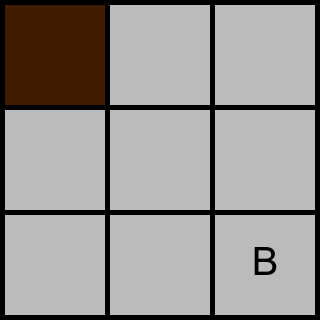
\includegraphics[width=\linewidth]{0.png}
\endminipage\hfill
\minipage{0.18\textwidth}
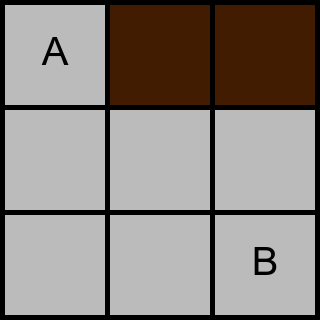
\includegraphics[width=\linewidth]{1.png}
\endminipage\hfill
\minipage{0.18\textwidth}
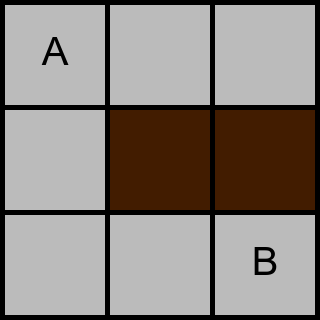
\includegraphics[width=\linewidth]{2.png}
\endminipage\hfill
\minipage{0.18\textwidth}
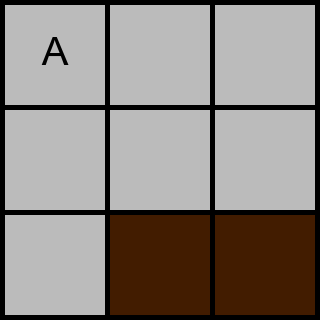
\includegraphics[width=\linewidth]{3.png}
\endminipage\hfill
\minipage{0.18\textwidth}
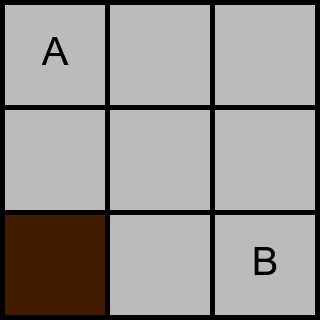
\includegraphics[width=\linewidth]{4.png}
\endminipage
\caption{Halva lösningen till det första exempelfallet. Rätblocket flyttas först ett steg till höger, sedan två steg nedåt och till sist ett steg åt vänster.}
\end{figure}

På mer avancerade nivåer i spelet så förekommer även så kallade \emph{modulo-celler}. Dessa är celler som kan befinna sig i två olika tillstånd, $0$ eller $1$. I tillstånd $0$ så beter sig en modulo-cell precis som en ledig cell som rätblocket kan röra sig på. I tillstånd $1$ så är dock modulo-celler upphöjda och beter sig som blockerade celler. Det kan även finnas växlar utplacerade på banan. När rätblocket ställs på en växel så ändras tillstånden på alla modulo-celler ($0$ blir till $1$ och vice versa).

\begin{figure}[!htb]
\minipage{0.45\textwidth}
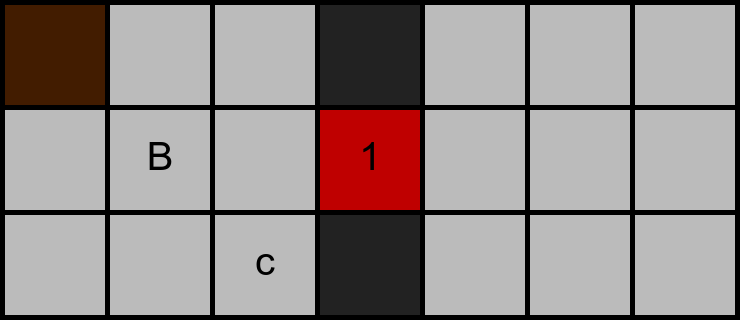
\includegraphics[width=\linewidth]{m0.png}
\endminipage\hfill
\minipage{0.45\textwidth}
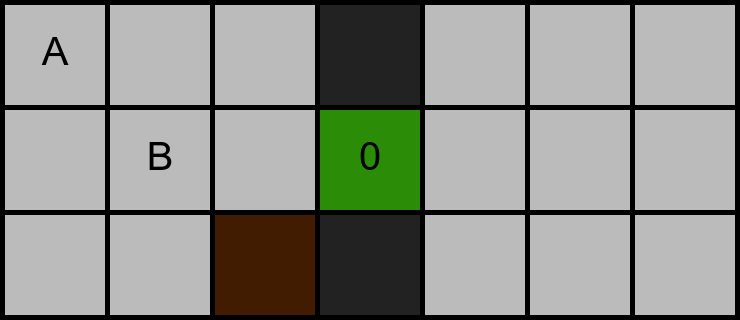
\includegraphics[width=\linewidth]{m1.png}
\endminipage
\caption{Det tredje exempelfallet, före och efter att växeln har aktiverats.}
\end{figure}

Banorna är designade så att det alltid finns en giltig lösning. Din uppgift är att beräkna det minsta antal förflyttningar som behövs för att lösa en bana.

\section*{Indata}

Du kommer först att få två heltal $N$ och $M$. Dessa betyder att banan har $N$ rader och $M$ kolumner.
De följande $N$ raderna har $M$ tecken var och beskriver hur banan ser ut. Följande tecken kan förekomma:

\begin{itemize}
\item $A$ eller $B$: beskriver banans start- respektive slut-positioner.
\item . (en punkt): beskriver en ledig cell.
\item \#: beskriver en blockerad cell.
\item $0$ eller $1$: beskriver en modulo-cell med givet start-tillstånd.
\item c: beskriver en växel
\end{itemize}

Det är garanterat att varje bana har precis ett $A$ och ett $B$.

\section*{Utdata}

Skriv ut en rad med ett heltal, det minsta antal förflyttningar som behövs för att flytta rätblocket från cell $A$ till cell $B$.

\section*{Poängsättning}

För testfall värda $2$ poäng så finns inga modulo-celler.
För de resterande $3$ poängen så behöver din lösning även kunna hantera modulo-celler.
